% !TeX root = status1.tex

\section{Preliminaries}
\label{sect-prelim}

\subsection{Boolean algebras}

\begin{definition}[Boolean algebra]
Let a set $B$ with two elements $\bot, \top \in B$ be given and operations ${\land}, {\lor} : B \times B \rightarrow B$ and ${\neg} : B \rightarrow B$. We call $(B,\bot,\top,\land,\lor,\neg)$ a \emph{Boolean algebra} iff  the following is satisfied for all $x, y, z \in B$:
\begin{itemize}
	\item ${\land}$ and $\lor$ are associative, commutative, and idempotent,
	\item $0$ is neutral for $\lor$ and $1$ is neutral for $\land$,
	\item $\land$ is distributive over $\lor$, and $\lor$ is distributive over $\land$,
	\item $x \lor 1 = 1$ and $x \land 0 = 0$,
	\item $x \lor (x \land y) = x = x \land (x \lor y)$,
	\item $x \land \neg x = 0$,
	\item $x \lor \neg x = 1$,
	\item $\neg \neg x = x$.
\end{itemize}
We abbreviate ``Boolean algebra'' with BA, and we call the operations \emph{connectives}. 
\end{definition}

We can impose a partial order on $B$ in a canonical way by defining:
\begin{equation*}
a \le b \Iff a \land b = a.
\end{equation*}

\begin{definition}[Atom]
An \emph{atom} of a Boolean algebra $B$ is an element $a\in B$ such that $a \ne \bot$ and such that there is no $b$ with $\bot < b < a$. Or, equivalently, if for all $b\in B$, either $b=\bot$ or $a \le b$. We denote the set of atoms of $B$ as $\mathfrak{A}_B$, or just $\mathfrak{A}$ when $B$ is clear from the context.
\end{definition}

We will repeatedly work with the free Boolean algebra $\mathcal{P}(X)$ generated by a finite set $X$, in which $\bot = \varnothing$, $\top = X$, $Y \land Z = Y \cap Z$, $Y \lor Z = Y \cup Z$ and $\neg Y = X \setminus Y$. The basis of this Boolean algebra consists of all singleton sets which are precisely the atoms.

\begin{example}
For any set $P$, we can build the \emph{free Boolean algebra with propositions $P$}. Valuations of the propositions are functions from $P$ to $2 = \{0 ,1\}$. We define $B = \mathcal{P}(2^P)$, and notice the atoms of $B$ are exactly the valuations.
\end{example}

An element $x$ of the free Boolean algebra with propositions $P$ is just a set of valuations which determine when $x$ is considered true. The usual set theoretic operations correspond with the logical connectives in this case. Now we study several useful elementary properties of Boolean algebras:

\begin{lem}
\label{and}
We have $\phi \leq \psi \wedge \chi$ iff $\phi \leq \psi$ and $\phi \leq \chi$ for any $\phi$, $\psi$ and $\chi$ in a Boolean algebra.
\end{lem}

\begin{proof}
Let $\phi, \psi, \chi$ be arbitrary elements in a Boolean algebra, and assume that $\phi \leq \psi$ and $\phi \leq \chi$. Then we have:
\[\phi \land \psi \land \chi = \phi \land \chi = \phi.\]
So, $\phi \leq \psi \land \chi$.

Now we assume that $\phi \leq \psi \land \chi$. Because $\psi \land \chi \leq \psi$ and $\psi \land \chi \leq \chi$, we see by transitivity of $\le$ that $\phi \leq \psi$ and $\phi \leq \chi$.
\end{proof}

\begin{lem}
\label{phi-psi}
In any Boolean algebra $B$ we have $\phi \land \psi = \phi$ iff $\phi \land \neg \psi = \bot$ for any two elements $\phi,\psi\in B$.
\end{lem}

\begin{proof}
For the one direction, assuming that $\phi \land \neg \psi = \bot$, we can compute:
\begin{equation*}
\begin{split} 
\phi \land \psi &= \bot \lor (\phi \land \psi)\\
&= (\phi \land \neg \psi) \lor (\phi \land \psi)\\
&= ((\phi \land \neg \psi) \lor \phi) \land ((\phi \land \neg \psi) \lor \psi)\\
&= (\phi \lor \phi) \land (\neg \psi \lor \phi) \land (\phi \lor \psi) \land (\neg \psi \lor \psi)\\
&= \phi \land (\phi \lor \neg \psi) \land (\phi \lor \psi) \land \top\\
&= \phi \land (\phi \lor (\neg \psi \land \psi))\\
&= \phi \land (\phi \lor \bot)\\
&= \phi \land \phi\\
&= \phi
\end{split}
\end{equation*}

For the other direction, we assume that $\phi \land \psi = \phi$, and can compute:
\[\phi \land \neg \psi = \phi \land \psi \land \neg \psi = \phi \land \bot = \bot.\]
Hence, $\phi \land \psi = \phi$ iff $\phi \land \neg \psi = \bot$.
\end{proof}

One can also characterize the notion of atoms:

\begin{lem}
\label{atom-char}
Let $B$ be any Boolean algebra, and let $a$ be any element. Then $a$ is an atom iff we either have $a \leq c$ or $a \leq \neg c$ for all $c \in B$.
\end{lem}

\begin{proof}
Assume that $a$ is an atom and $a \land c \leq a$, we know $a \land c = a$ or $a \land c = \bot$. In the first case, we have by definition $a \leq c$. In the second case we have by Lemma \ref{phi-psi} $a \leq \neg c$.

Now we assume that $a \leq c$ or $a \leq \neg c$ for every $c \in B$. Let $b \leq a$ be any element, and now we claim $b \in \{a, \bot\}$ which says $b$ is an atom. Then we have either $a \leq b$ or $a \leq \neg b$. In the first case we have $a = b$. In the second case we have by combining the definition and Lemma \ref{phi-psi} that $b = a \land b = \bot$. Hence, $a$ is an atom.
\end{proof}

\begin{lem}
Given a Boolean algebra $B$, an atom $a$ and elements $b, c \in B$ such that $a \leq b \lor c$, then we have $a \leq b$ or $a \leq c$.
\end{lem}

\begin{proof}
By the previous lemma we either have $a \leq b$ or $a \leq \neg b$. In the first case it holds, so now we assume $a \leq \neg b$. This means that $a \land b = \bot$ by Lemma \ref{phi-psi}. Now we see:
\[a \land \neg c = a \land (b \lor c) \land \neg c = (a \land b \land \neg c) \lor (a \land c \land \neg c) = \bot \lor \bot = \bot.\]
Hence, $a \leq c$. 
\end{proof}

Lastly, we introduce several algebraic notions.

\begin{definition}[Subalgebra]
\label{subalgebra}
Let a Boolean algebra $B$ and a subset $C \subseteq B$ be given. We call $C$ a \emph{subalgebra} of $B$ iff $\bot, \top \in C$, and $C$ is closed under the Boolean algebraic operations, that is, whenever $a, b \in C$, we have $\neg a \in C$, $a \land b \in C$ and $a \lor b \in C$.
\end{definition}

We will not prove the following proposition, and just remark that it can be proven in a similar way as the analogous statement for groups, rings or modules.

\begin{proposition}
\label{intersection}
The intersection of an arbitrary set of subalgebras of any Boolean algebra is again a subalgebra.
\end{proposition}

\begin{definition}[Generated subalgebra]
\label{gen-sub}
Let $B$ be a Boolean algebra and let $C$ be a subset of $B$. We call the \emph{generated subalgebra} of $C$ as the intersection of all subalgebras containing $C$, and we denote this subalgebra by $\langle C \rangle$.
\end{definition}

Notice that by Proposition \ref{intersection} the generated subalgebra is indeed a subalgebra. Furthermore, the elements of the generated subalgebra $C$ are combinations of elements in $C$.

\begin{proposition}
\label{subalgebra-induc}
Let $B$ be any Boolean algebra with any subset $C$, define $A_0 = C$ and $A_{n+1} = A_n \cup \{x \lor y : x, y \in A_n \} \cup \{x \land y : x, y \in A_n \} \cup \{\neg x : x \in A_n \}$, and let $A = \bigcup_{i=0}^\infty A_i$. Then we have $\langle C \rangle = A$.
\end{proposition}

\begin{proof}
First, we prove that $A$ is a subalgebra, in which case we know that $\langle C \rangle \subseteq A$, by definition of $\langle C \rangle$ being the intersection of all subalgebras. Take any $x, y \in A$ arbitrarily. Then we have $x \in A_n$ and $y \in A_m$ for some $n, m \in \mathbb{N}$. Let $k = \max(n, m)$, and by construction we have $x, y \in A_k$. Hence, we can conclude $x \lor y, x \land y, \neg x \in A_{k+1} \subseteq A$. Therefore, we can conclude $A$ is a subalgebra, and thus $\langle C \rangle \subseteq A$.

Now we prove that $A \subseteq \langle C \rangle$. By induction we show that for every $n \in \mathbb{N}$ we have $A_n \subseteq \langle C \rangle$, in which case indeed $A = \bigcup_{i=0}^\infty A_i \subseteq \langle C \rangle$. First, we notice that $A_0 = C \subseteq \langle C \rangle$. Now we assume that $A_n \subseteq \langle C \rangle$, and take $x \in A_{n+1}$ arbitrary. By construction we can either write $x = a \lor b$, $x = a \land b$ or $x = \neg a$ with $a, b \in A_{n+1} \subseteq \langle C \rangle$. Because $\langle C \rangle$ is a subalgebra, we must have that $x \in \langle C \rangle$. Therefore, we can conclude that $A \subseteq \langle C \rangle$. Hence, $A = \langle C \rangle$, because $\langle C \rangle$ is the intersection of all subalgebras and therefore contains $A$ as well.
\end{proof}

The proposition says that we can construct the smallest subalgebra of any subset $C$ by taking combinations of elements in $C$. However, these combinations can be arbitrary long, so we use induction to get every combination. 

For the rest of this report we will mostly concern ourselves with Boolean algebras generated by a finite set of propositions.

\subsection{Minterms}

\citep{veanes} introduces a notion of \emph{minterms} to optimize a proposed minimization algorithm for symbolic finite automata (which will be introduced later).

Veanes defines minterms by giving the computing algorithm, which is included below:

\algloopdefx{NoEndIf}[1]{\textbf{if} #1 \textbf{then}}
\begin{algorithm}
\caption{Veanes' minterms algorithm}
\vspace*{3pt}
\begin{minipage}[t]{.5\textwidth}
\begin{algorithmic}[1]
\Function{Minterms}{BA $B$, $\{c_1 \dots c_n\}\subseteq B$}
\State $\textit{tree} := $ \textbf{new} \textsc{TreeNode}($\top$)
\For {$i=1\dots n$}
  \For {$\ell \in $ \textsc{Leaves}($\textit{tree}$)}
    \State $\ell$.\textsc{Add}($c_i$)
  \EndFor
\EndFor
\EndFunction
\end{algorithmic}
\end{minipage}
\begin{minipage}[t]{.5\textwidth}
\begin{algorithmic}[1]
\Class~\textsc{TreeNode}($\phi$)
\State \textsc{TreeNode} \textit{left} $:=$ \textsc{Null}
\State \textsc{TreeNode} \textit{right} $:=$ \textsc{Null}
\Function{Add}{$\psi$}
\If{$\phi \land \psi \ne \bot$ \textbf{and} $\phi \land \neg\psi \ne \bot$}
  \State$\textit{left} := $ \textbf{new} \textsc{TreeNode}($\phi \land \psi$)
  \State$\textit{right} := $ \textbf{new} \textsc{TreeNode}($\phi \land \neg\psi$)
\EndIf
\EndFunction
\EndClass
\end{algorithmic}
\end{minipage}
\vspace*{3pt}
\end{algorithm}

We give the following mathematical analog to the algorithm:

\begin{definition}[Minterms]
Let $C = \{c_1, ..., c_n\}$ be any finite subset of a Boolean algebra $B$. For every $1 \leq i \leq n$ we define a function $f_i : B \rightarrow \mathcal{P}(B)$ by
\begin{equation*}
f_i(x) = \begin{cases} \{x\} & \text{if $x \land c_i = \bot$ or $x \land \neg c_i = \bot$} \\ \{x \land c_i, x \land \neg c_i\} & \text{otherwise}\end{cases}
\end{equation*}
Then we define intermediate step minterms as
\begin{align*}
M_0(C) &= \{\top\}, \\
M_i(C) &= f_i[M_{i-1}], \quad \text{for every $1 \le i \le n$}.
\end{align*}
Finally the set of \emph{minterms} of $C$ is the set $M(C) := M_n(C)$.
\end{definition}

Notice that this definition implicitly assumes that $C$ is ordered. This is possible, since any finite set can be ordered. However, it might not be well-defined for arbitrary sets. With that issue we will deal later.

This definition corresponds to the execution of Veanes' algorithm in \citep{veanes}. This algorithm iteratively builds a tree whose leaves are precisely the minterms. The root node of the tree is ${\top}$. If we have built the tree up to a certain level $k$, we have only used the elements $c_1, ..., c_k$ of $C$. Dealing with the new element $c_{k+1}$, we consider every leaf node $\ell$ of the current tree. If $\ell \land c$ and $\ell \land \neg c$ are both unequal to $\bot$, we add them as children to $\ell$, and else just let $\ell$ be.

\begin{example}
As an example, consider computing the minterms for $C = \{c_1 = a, ~c_2 = a\lor b, ~c_3 = a\land (b\lor c)\}$, shown diagrammatically below:

% easy tikz trees:
%   http://www.ctan.org/pkg/tikz-qtree
% vertically align trees to top:
%   http://tex.stackexchange.com/questions/100870/how-to-horizontally-top-align-multiple-tikzpictures-without-using-hspace
\begin{table}[h]
\centering
\begin{tabu}{c|c|c|c}
\rowfont[c]{\bfseries}
step 0 & step 1 & step 2 & step 3 \\
\midrule
\raisebox{-\height}{\begin{tikzpicture}
\Tree
[.$\top$ ]
\end{tikzpicture}}
&
\raisebox{-\height}{\begin{tikzpicture}
\Tree
[.$\top$
  [.$a$ ]
  [.$\neg a$ ]
]
\end{tikzpicture}}
&
\raisebox{-\height}{\begin{tikzpicture}
\Tree
[.{$\top$}
  [.{$a$} ]
  [.{$\neg a$}
    [.{$\neg a \land b$} ]
    [.{$\neg a \land \neg b$} ]
  ]
]
\end{tikzpicture}}
&
\raisebox{-\height}{\begin{tikzpicture}
\Tree
[.{$\top$}
  [.{$a$}
    [.{$a \land (b \lor c)$} ]
    [.{$a \land \neg b \land \neg c$} ]
  ]
  [.{$\neg a$}
    [.{$\neg a \land b$} ]
    [.{$\neg a \land \neg b$} ]
  ]
]
\end{tikzpicture}}
\end{tabu}
\end{table}
\end{example}

By induction we can see that the set of minterms of some set $C$ corresponds to the given definition. If $C$ is empty, the tree consist of just a node ${\top}$, and this will be the only minterm. If we have computed the minterms of a set $\{c_1, ..., c_n\}$ and we have an element $c_{n+1}$, then the minterms of $\{c_1, ..., c_n, c_{n+1}\}$ are precisely given by the definition. If we have a leaf node $\ell$, then it is a minterm if no child is added (so, if $\ell \land c_{n+1} = \bot$ or if $\ell \land \neg c_{n+1} = \bot$). However, if children are added to $\ell$, then it gives two minterms, namely $x \land c_i$ and $x \land \neg c_i$. The algorithm takes $n$ steps, so the final result is $M_{n}(C)$, and thus we can define the minterms of $C$ as $M_{n}(C)$.

\begin{lem}
\label{write-as-minterms-disjunction}
Let $C = \{c_1, ..., c_n\}$ be any finite subset of a Boolean algebra $B$. Then every $c \in M_i(C)$ can be written as a disjunction of minterms.
\end{lem}

\begin{proof}
For this proof we use downward induction. If $c \in M_{n+1}(C)$, then $c$ is a minterm. Assume the proposition holds for every element in $M_{n+1}(C)$, and take $c \in M_{n}(C)$ arbitrary. By construction of $M_{n+1}(C)$, we either have that $c \in M_{n+1}(C)$ or that $c \land c_i, c \land \neg c_i \in M_{n+1}(C)$. In the first case we can write $c$ as a disjunction of minterms by the induction hypothesis. In the second case, we write both $c \land c_i$ and $c \land \neg c_i$ as a disjunction of minterms, and we notice that $c = c \land \top = c \land (c_i \lor \neg c_i) = (c \land c_i) \lor (c \land \neg c_i)$ is a disjunction of minterms as well. 
\end{proof}

\begin{lem}
Let $C = \{c_1, ..., c_n\}$ be any finite non-empty subset of a Boolean algebra $B$. Then $\top$ can be written as a disjunction of minterms.
\end{lem}

\begin{proof}
This follows from Lemma \ref{write-as-minterms-disjunction}, because $\top \in M_0(C)$.
\end{proof}

By looking at the proof in more detail, one sees that $\top$ is the disjunction of all minterms. This can be proven with a similar induction argument.

\begin{lem}
Let $C = \{c_1, ..., c_n\}$ be any finite non-empty subset of a Boolean algebra $B$, and let $m, n \in M(C)$ be distinct minterms. Then $m \land n = \bot$.
\end{lem}

\begin{proof}
We use induction. If $n = 1$, we have $M(C) = \{c_1, \neg c_1\}$, and then it holds. Assume, it holds for some $n$. A minterm of $\{c_1, ..., c_n, c_{n+1}\}$ is a conjunction of a minterm of $\{c_1, ..., c_n\}$ and $c_{n+1}$ or $\neg c_{n+1}$. So, let $m$ and $n$ be arbitrary minterms. There are two cases now: we can either write $m = c_i \land c_{n+1}$ and $n = c_j \wedge d$ where $i \neq j$ and $d \in \{c_{n+1}, \neg c_{n+1}\}$ or we can write $m = c_i \land c_{n+1}$ and $n = c_i \wedge \neg c_{n+1}$. In the first case we have $m \land n = \bot$ by the induction hypothesis, and in the second case we have $m \land n = \bot$, because $c_{n+1} \land \neg c_{n+1} = \bot$. Therefore, the proposition holds for all finite non-empty sets.
\end{proof}

\begin{lem}
Let $C = \{c_1, ..., c_n\}$ be any finite subset of a Boolean algebra $B$. Then every $c_i$ can be written as combination of minterms of $C$.
\end{lem}

\begin{proof}
Let $c_i$ be any element. With induction we can prove $M_{i-1}$ is not empty. Now there are two cases: there either is an $x \in M_{i-1}(C)$ such that $x \land c_i \neq \bot$ and $x \land \neg c_i \neq \bot$, or this is not the case. In the first case we can write:
\[x = x \land \top = x \land (c_i \lor \neg c_i) = (x \land c_i) \lor (x \land \neg c_i).\]
Because $x \land c_i \neq \bot$ and $x \land \neg c_i \neq \bot$, we know that both are elements of $M_i(C)$, and thus they can be written as a combination of minterms by Lemma \ref{write-as-minterms-disjunction}. Hence, $x$ can be written as combination of minterms.

Now we assume that for all $x \in M_{i-1}(C)$ we have $x \land c_i = \bot$ or $x \land \neg c_i = \bot$. Denote $X = \{x \in M_{i-1}(C) : x \land \neg c_i = \bot\}$, and let $Y = M_{i-1}(C)-X$. Now we see that $\top = (\bigvee_{x \in X} x) \vee \bigvee_{y \in Y} y$, that $c_i \wedge y = \bot$ for any $y \in Y$ by assumption and that $x \in X$ iff $x \leq c_i$ by Lemma \ref{phi-psi} we see that $x \in X$ iff $x \leq c_i$. Using that we compute:
\begin{equation*}
\begin{split}
c_i &= c_i \land \top\\
&= c_i \land ((\bigvee_{x \in X} x) \vee \bigvee_{y \in Y} y)\\
&= (\bigvee_{x \in X} c_i \land x) \vee (\bigvee_{y \in Y} c_i \land y)\\
&= (\bigvee_{x \in X} c_i \land x) \vee \bigvee_{y \in Y} \bot\\
&= \bigvee_{x \in X} c_i \land x\\
&= \bigvee_{x \in X} x
\end{split}
\end{equation*}
Therefore, every element of $C$ can be written as combination of minterms.
\end{proof}

The set $X$ in the previous lemma is interesting. We see that $x \in X$ if and only if $x \leq c_i$. This says that an element of $C$ is described by the minterms below it.

By combining the previous lemmas we get the following:

\begin{proposition}
\label{minterms-props}
For every finite subset $C\subseteq B$ the following holds:
\begin{enumerate}
\item for every $m,m'\in M(C)$ we have $m\land m' = \bot$;
\item every $c \in C$ can be written as $c = \bigvee X$ for some $X \subseteq M(C)$;
\item $\bigvee M(C) = \top$;
\item $M(C)$ does not include ${\bot}$.
\end{enumerate}
\end{proposition}

If we have $m \land m' = \bot$, we say that $m$ and $m'$ are \emph{mutually exclusive}. Furthermore, these results can be used to prove that every finite subalgebra of a Boolean algebra is free.

\begin{proposition}
\label{finite-free-sub-is-free}
Any finite subalgebra $C$ of a Boolean algebra $B$ is free.
\end{proposition}

\begin{proof}
Let $B$ be any Boolean algebra and let $C = \{c_1, ..., c_n\}$ be a subalgebra of $B$. Our goal is to prove that $C$ is free, and for that we prove that $C$ is isomorphic to the Boolean algebra $\mathcal{P}(M(C))$. We define a map $f : C \rightarrow \mathcal{P}(M(C))$ as $f(x) = \{m \in M(C) : m \leq x\}$. Now we prove $f$ is an isomorphism. 

First, we prove that $f$ is a homomorphism. Let $a$ and $b$ be arbitrary elements of $C$. Then we have by Lemma \ref{and}:
\[f(a \land b) = \{m \in M(C) : m \leq a \land b\} = \{m \in M(C) : m \leq a\} \cap \{m \in M(C) : m \leq b\} = f(a) \cap f(b),\]
\[f(a \lor b) = \{m \in M(C) : m \leq a \lor b \} = \{m \in M(C) : m \leq a\} \cup \{m \in M(C) : m \leq b\}.\]

For this proof, let variables $m$ and $m'$ always run over $M(C)$.

We know $a \leq a \lor b$ and $b \leq a \lor b$, so if $m \leq a$ or $m \leq b$, we must have $m \leq a \lor b$. Next we assume $m \leq a \lor b$, and we write $a = \bigvee_{m' \le a} m'$ and $b = \bigvee_{m' \leq b} m'$. Then we have $m \le (\bigvee_{m' \leq a} m') \lor \bigvee_{m' \leq b} m'$. This means $m = m \land ((\bigvee_{m' \leq a} m') \lor \bigvee_{m' \leq b} m') = (\bigvee_{m' \leq a} m \land m') \lor (\bigvee_{m' \leq b} m \land m')$. If neither $m \leq a$ nor $m \leq b$ hold, then we have
\[m = (\bigvee_{m' \leq a} m \land m') \lor (\bigvee_{m' \leq b} m \land m') = \bot \lor \bot = \bot,\]
because minterms are mutually exclusive. However, we have $m \neq \bot$, because $m$ is a minterm. So, either $m \leq a$ or $m \leq b$.

If we have $m \leq \neg a$, then $m=m \land \neg a$. Then we cannot have that $m=m \land a$, because then we have:
\[m=m \land a = m \land \neg a \land a = \bot.\]
Because $m$ is a minterm, we know $m \neq \bot$. We know $m \leq \top = a \lor \neg a$, and by the previous reasoning we see that either $m \leq a$ or $m \leq \neg a$. Therefore, we must have $m \leq a$. Now we can conclude
\[f(\neg a) = \{m \in M(C) : m \leq \neg a\} =  \mathcal{P}(M(C)) \setminus \{m \in M(C) : m \leq a\}.\]
Hence, $f$ is a homomorphism.

To see that $f$ is injective, assume $f(a) = f(b)$. Then we have:
\[a = \bigvee_{m \leq a} m = \bigvee_{m \in f(a)} m = \bigvee_{m \in f(b)} m = \bigvee_{m \le b} m = b.\]

Now we prove $f$ is surjective. Since we know $f(m) = \{m\}$ for any minterm $m$ and that $f$ is a homomorphism, we see that:
\[\{m_1, ..., m_k\} = \bigcup_{i=1}^k \{m_i\} = \bigcup_{i=1}^k f(m_i) = f(\bigvee_{i=1}^km_i).\]
Hence, $f$ is a bijection, and thus an isomorphism.
\end{proof}

The previous proposition tells us that the atoms of $C$ are precisely the minterms of $C$, and that $C$ is free. Now we extend these results for arbitrary sets:

\begin{proposition}
\label{minterms-generated}
Let $C$ be an arbitrary finite subset of a Boolean algebra $B$. Then we have $M(C) = M( \langle C \rangle )$.
\end{proposition}

\begin{proof}
If $C = \emptyset$, $C = \{\top, \bot\}$ or $C = \{\bot\}$, we have $M(C) = \{\top\}$ and $\langle C \rangle = \{\top, \bot\}$. Therefore, we can assume there is a $c \in C$ such that $c \notin \{\top, \bot\}$. Let $F = \langle M(C) \rangle$ be the smallest subalgebra containing $M(C)$. Notice that every element of $F$ can be written as a combination of minterms of $C$, and that $C \subseteq F$. Notice $\langle C \rangle \subseteq F$, because $\langle C \rangle$ is the smallest subalgebra containing $C$. Since elements of $M(C)$ are combinations of elements in $C$, we know $M(C) \subseteq \langle C \rangle$. Since $F$ is generated by $M(C)$, we therefore must have that $F = \langle C \rangle$. Therefore, the atoms of $F$ and $\langle C \rangle$ must be equal, so it is sufficient to prove the atoms of $F$ are precisely $M(C)$.

First, we prove every element $m \in M(C)$ is an atom of $F$. For that, we use Lemma \ref{atom-char}, and we fix any $m \in M$. Notice that $F$ is built inductively by Proposition \ref{subalgebra-induc}, and with induction we prove for every $c \in F$ we have $m \leq c$ or $m \leq \neg c$. First, we assume $c$ is a minterm. If $c = m$, we have $m \leq c$. If $c \neq m$, we have $m \leq \neg c$, because $m \land c = \bot$. For the induction step we have multiple cases:

\begin{itemize}
	\item Assume, $c = a \lor b$, and it holds for $a$ and $b$. This means we have $m \leq a$ or $m \leq \neg a$, and $m \leq b$ or $m \leq \neg b$. If $m \leq a$ or $m \leq b$, we see $m \leq a \lor b$. If $m \leq \neg a$ and $m \leq \neg b$, then we have $n \leq \neg a \land \neg b = \neg (a \lor b)$. 
	\item Next we suppose $c = a \land b$, thus we have $m \leq a$ or $m \leq \neg a$, and $m \leq b$ or $m \leq \neg b$. If $m \leq a$ and $m \leq b$, then we have $m \leq a \land b$. If $m \leq \neg a$ or $m \leq \neg b$, then we have $m \leq \neg a \lor \neg b = \neg (a \land b)$.
	\item Lastly, assume that $c = \neg a$, and that $m \leq a = \neg \neg a$ or $m \leq \neg a$.  
\end{itemize}

Hence, we can conclude every $m \in M(C)$ is an atom of $F$.

Next we prove every atom is an element of $M(C)$, and then we can conclude the atoms of $F$ is $M(C)$. For this we prove every element of $F$ is the disjunction of all minterms below it. From this we can conclude that the atoms are contained in $M(C)$. Let $a \neq \bot$ be any atom of $F$. Then $a \in A_n$ for some $a$, so we can find $m$ such that $m \leq a$, because $a \neq \bot$. Because $a$ is an atom, we must have $m = a$, thus $a$ must be a minterm.

Now we prove with induction that every element is the disjunction of the minterms below it. If $c$ is any minterm, then the only minterm $m'$ with $m' \leq c$ is $c$, and $c = c$, so it holds. For the induction step we have multiple cases.

\begin{itemize}
	\item Suppose that $c = a \lor b$, and write $a = \bigvee_{m \leq a} m$ and $b = \bigvee_{m \leq b} m$. Because for every $m$ with $m \leq a$ or $m \leq b$ we have $m \leq a \lor b$, and because $c = \bigvee_{m \leq a} m \vee \bigvee_{m \leq b} m$, we can conclude $c = \bigvee_{m \leq a \lor b} m$. 
	\item Next we assume $c = a \land b$, and we write $a = \bigvee_{m \leq a} m$ and $b = \bigvee_{m \leq b} m$. Now we see:
	\[c = (\bigvee_{m \leq a} m) \land \bigvee_{m \leq b} m = \bigvee_{m \leq a} \bigvee_{m' \leq b} m \land m'.\]
	We have $m \land m' = \bot$ if $m \neq m'$, so we see $c = \bigvee_{m \leq a \land b} m$.
	\item Lastly, let $c = \neg a$, and assume $a = \bigvee_{m \leq a} m$. Let $X = \{m \in M(C) : m \leq a\}$ and $Y = \{m \in M(C) : m \not \leq a\}$, and notice that $X \cup Y = M(C)$. Now we see that $\bigvee_{m \in X} m = a$ and $\bigvee_{m \in X \cup Y} m = \top$. Also, notice that $m \leq \neg a$ if $m \in Y$. Therefore, we can conclude that $\bigvee_{m \in Y} m \leq \neg a$. Furthermore, we have $\top = a \lor \bigvee_{m \in Y} m$. Hence, we have
	\[\neg a \land \neg \bigvee_{m \in Y} m = \neg (a \lor \bigvee_{m \in Y} m) = \neg \top = \bot.\]
	Therefore, $\neg a \leq \bigvee_{m \in Y} m$, so we can conclude $\neg a = \bigvee_{m \in Y} m$.
\end{itemize}
Hence, we can conclude every element is the disjunction of minterms below it.
\end{proof}

\begin{proposition}
Let $\{c_1, ..., c_n\}$ be any subset of a Boolean algebra $B$, and let $\sigma$ be any permutation of $\{1, ..., n\}$. Then we have $M(\{c_1, ..., c_n\} = M(\{c_{\sigma(1)}, ..., c_{\sigma(n)}\})$.
\end{proposition}

\begin{proof}
The minterms are by Proposition \ref{minterms-generated} the atoms of the generated subalgebra, and these do not depend on the total order of the Boolean algebra. Therefore, we must have that $M(\{c_1, ..., c_n\} = M(\{c_{\sigma(1)}, ..., c_{\sigma(n)}\})$.
\end{proof}

Now we can conclude the generated subalgebra of any subset $C$ is free, and the atoms are $M(C)$. Also, we have $\langle C \rangle = \mathcal{P}(M(C))$. Next we see the minterms induce a relation on the atoms of the Boolean algebra.

\begin{definition}[Induced relation]
Given a finite subset $C$ of a free Boolean algebra $B$, we define the \emph{induced relation} ${\sim}_{M(C)} \subseteq A_B \times A_B$ and we say $a \sim a'$ iff there is a $m \in M(C)$ such that $a \le m\land a' \le m$. If the set $C$ is clear from the context, we leave out the subscript.
\end{definition}

With induction we see that if $a \leq \bigvee_{i=1}^n b_i$, we must have $a \leq b_i$ for some $i$.

\begin{proposition}
The induced relation $\sim_{M(C)}$ is an equivalence relation where $C$ is a finite subset of a Boolean algebra $B$.
\end{proposition}

\begin{proof}
For the proof we have to show ${\sim}$ is reflexive, symmetrical and transitive. 

\begin{description}
\item[Reflexivity] We have to prove that for every atom $a$ there is a minterm $m$ such that $a \leq m$. Notice that $a \leq \top$, and that $\top$ can be written as disjunction of minterms. Hence, by the previous lemmas there must be an $m$ such that $a \leq m$.

\item[Symmetry] If there is a $m$ such that $a \leq m$ and $a' \leq m$, then we can conclude $a' \sim a$. 

\item[Transitivity] Suppose that $a \sim b$ and $b \sim c$. Because $b$ is an atom, we have $b \neq \bot$. Furthermore, we have $m,m'\in M(C)$ such that $a\le m$, $b \le m$, $b \le m'$ and $c \le m'$. This implies that $b \le m \land m'$, and we must have $m = m\land m' = m'$, because minterms are mutually exclusive. Hence, $a \sim c$.
\end{description}
Therefore, we can conclude ${\sim}$ is an equivalence relation.
\end{proof}

If $B$ is a Boolean algebra generated by a finite set of proposition, the atoms are the valuations. This means the minterms partition the valuations.

\begin{example}
In this example we see how the minterms of our earlier set $C = \{a, a\lor b, a\land (b\lor c)\}$ indeed partitions the valuation space of the free Boolean algebra with propositions $a$, $b$ and $c$.
\begin{equation*}
\begin{tikzpicture}
\tikzset{frontier/.style={distance from root=110pt}}
\Tree
[.{$\top$}
  [.{$a$}
    [.{$a \land (b \lor c)$}
      {\begin{tabular}{c}
        101 \\
        110 \\
        111
      \end{tabular}} ]
    [.{$a \land \neg b \land \neg c$}
      {\begin{tabular}{c}
        100 \\
        ~ \\
        ~
      \end{tabular}} ]
  ]
  [.{$\neg a$}
    [.{$\neg a \land b$}
      {\begin{tabular}{c}
        010 \\
        011 \\
        ~
      \end{tabular}} ]
    [.{$\neg a \land \neg b$}
      {\begin{tabular}{c}
        000 \\
        001 \\
        ~
      \end{tabular}} ]
  ]
]
\end{tikzpicture}
\end{equation*}
\end{example}

\subsection{Automata}

We start with the usual definitions of automata.

\begin{definition}[Nondeterministic Finite Automaton]
A \emph{nondeterministic finite automaton} over an alphabet $\Sigma$ is a structure $(Q,F,\Delta)$, where $Q$ is a finite set and $F\subseteq Q$.  We call elements of $Q$ the \emph{states} and elements of $F$ the \emph{final states}. Also, $\Delta : Q \times \Sigma \to Q$ is called the \emph{transition function}, and we write $q \trans{a} q'$ iff $\Delta(q, a, q')$. Lastly, we abbreviate ``deterministic finite automaton'' as NFA, and the class of all NFAs is denoted as $\mathcal{N}$.
\end{definition}

\begin{definition}[Deterministic Finite Automaton]
A \emph{deterministic finite automaton} over an alphabet $\Sigma$ is an NFA $(Q,F,\Delta)$ such that $\Delta$ is a function. We ``abbreviate deterministic finite automaton'' as DFA, and we denote the class of all DFAs as $\mathcal{D}$.
\end{definition}

\begin{definition}[Language of an NFA]
Let $M$ be an arbitrary NFA. We define the \emph{language} $\operatorname{NL}_M : Q \to \mathcal{P}(\Sigma^*)$ \emph{accepted by $M$} as follows:
\begin{align*}
\varepsilon \in \operatorname{NL}_M(q) &\text{ iff } q \in F, \\
aw \in \operatorname{NL}_M(q) &\text{ iff there is } q' \text{ such that } q \trans{a} q' \text{ and } w \in \operatorname{NL}_M(q').
\end{align*}
\end{definition}

The automaton is parameterized in the definition of the language. Given any state, the language function determines a set of words, and those words are said to be accepted by the automaton. Now we consider a new class of automata:

\begin{definition}[Symbolic Finite Automaton]
A \emph{symbolic finite automaton} $M = (Q, F, \Delta)$ is an NFA over a set $B$ which is the free Boolean algebra for a finite set of propositions $P$. We define a relation $\Trans{} \subseteq Q \times A_B \times Q$ by
$q \Trans{a} q'$ iff there is a $\phi \ge a$ such that $q \trans{\phi} q'$. ``Symbolic finite automaton'' is abbreviated SFA, and the class of all symbolic finite automata is denoted as $\mathcal{S}$.
\end{definition}

The relation $\Trans{}$ is an alternative transition, or acceptence, relation. Transitions of the NFA go from a certain state to another state with some formula. However, our goal is to define the language with words of atoms which can be seen as the basic valuations of the Boolean algebra. Therefore, we need another relation which uses atoms instead of formulas. Such a transition can be taken precisely if the formula satisfies the valuation, and this means that it is greater than the atom in terms of ${\le}$.

There is no essential difference between de definition of SFAs and NFAs. Instead, the difference between the two types of automata is in how they accept languages. An NFA over a certain alphabet accepts words from that alphabet, but for a SFA we have more structure on the alphabet, and instead accept words of atoms, in terms of the alternative transition (or acceptance) relation.

\begin{definition}[Language of an SFA]
For an arbitrary SFA $M = (Q, F, \Delta)$ over an alphabet $B$ we define the \emph{(symbolic) language} $\operatorname{SL}_M : Q \to \mathcal{P}({A_B}^*)$ \emph{accepted by $M$} as:
\begin{align*}
\varepsilon \in \operatorname{SL}_M(q) &\text{ iff } q \in F, \\
aw \in \operatorname{SL}_M(q) &\text{ iff there is } q' \text{ such that } q \Trans{a} q' \text{ and } w \in \operatorname{SL}_M(q').
\end{align*}
\end{definition}

This definition is thus similar to the language of a NFA, but the alternative relation is used.

As SFAs are just NFAs with additional structure, we can forget this additional structure and use existing language equivalence deciding methods on SFAs. However, because SFAs accept languages in a different way, such an application needn't be meaningful. In fact, if two SFAs are determined to be language equivalent by a method for NFAs, then this result will be valid, but if the method determines them to have different languages, the additional structure of the SFAs might turn out to yield them to have the same (SFA) languages after all. That is, an NFA language equivalence deciding method is always sound, but not complete. More precisely, if $\mathcal{A}$ is an NFA language equivalence deciding method, i.e.~$\NL_M(q) = \NL_M(q')$ iff $\mathcal{A}_M(q,q')$, then for SFAs $M$ we only have one direction in general: $\SL_M(q) = \SL_M(q')$ implies $\mathcal{A}_M(q,q')$.

\begin{example} As an example, consider the following two SFAs:

\begin{equation*}
\begin{tikzpicture}[shorten >=1pt,node distance=2cm,on grid,auto]
   \node[state,accepting] (q_0) {$0$}; 
    \path[->]
    (q_0) edge [loop above] node {$\bot$} (q_0);
\end{tikzpicture}
\qquad\qquad
\begin{tikzpicture}[shorten >=1pt,node distance=2cm,on grid,auto]
   \node[state,accepting] (q_0) {$0$}; 
\end{tikzpicture}
\end{equation*}

If we consider these automata as normal NFAs ($\Sigma = B$, each formula is a different letter), their languages are $\{\bot^n : n \in \mathbb{N}\}$ and $\{ \varepsilon \}$, respectively. However, if we consider them as SFAs, both accept the same language, namely the language with only the empty word.
\end{example}

\subsection{Deciding language equivalence with Hopcroft-Karp}

Hopcroft-Karp (or HK) is an algorithm for deciding language equivalence of automata. It originally works only on deterministic automata, but can be efficiently applied to NFA as well by expanding the NFA to a DFA ``on the fly'', as explained in \citep{hkc}.

Note that instead of checking whether two automata with initial states have the same language, it is equivalent to ask whether two states in the same automaton have the same language, as one can just ``merge'' the two automata together.

Given a pair of states in a DFA, HK traverses the automaton in a forward fashion, iteratively collecting pairs of states that can be reached from previous pairs by some letter in the alphabet. If a pair of a final state together with a non-final state is found, we can conclude that all pairs previously collected accept different languages, and in particular the initial two states accept different languages, so the algorithm returns FALSE. Else, the algorithm returns TRUE.

The code of a slightly optimized version of the algorithm, called HKC where the ``C'' stands for a ``congruence'' relation as explained in \citep{hkc}, is given below. Applying HKC ``on the fly'' to an NFA, instead of pairs of states, we collect pairs of sets of states---following the canonical powerset construction for transforming a DFA to an NFA.

\algloopdefx{NoEndIf}[1]{\textbf{if} #1 \textbf{then}}
\begin{algorithm}
\caption{Hopcroft-Karp w/ congruence, for DFA resp.~NFA}
\vspace*{3pt}
\begin{minipage}{.5\textwidth}
\begin{algorithmic}[1]
\Function{\HK}{DFA $M$, $x,y\in Q_M$}
\State $R := \emptyset$
\State $\textit{todo} := \{(x,y)\}$
\While {$\textit{todo} \ne \emptyset$}
  \State extract $(x',y')$ from $\textit{todo}$
  \NoEndIf{$(x',y') \in e(R)$} \State \textbf{skip}
  \NoEndIf{$x' \in F_M$ \textbf{xor} $y' \in F_M$} \State \textbf{return} FALSE
  \For{$a \in \Sigma$}
    \State insert $(\Delta_M(x',a), \Delta_M(y',a))$
    \State \quad into $\textit{todo}$
  \EndFor
  \State insert $(x',y')$ into $R$
\EndWhile
\State \textbf{return} TRUE
\EndFunction
\end{algorithmic}
\end{minipage}
\begin{minipage}{.5\textwidth}
\begin{algorithmic}[1]
\Function{\HKND}{NFA $M$, $X,Y \subseteq Q_M$}
\State $R := \emptyset$
\State $\textit{todo} := \{(X,Y)\}$
\While {$\textit{todo} \ne \emptyset$}
  \State extract $(X',Y')$ from $\textit{todo}$
  \NoEndIf{$(X',Y') \in c(R \cup \textit{todo})$} \State \textbf{skip}
  \NoEndIf{$X' \in F_{\overline{M}}$ \textbf{xor} $Y' \in F_{\overline{M}}$} \State \textbf{return} FALSE
  \For{$a \in \Sigma$}
    \State insert $(\Delta_{\overline{M}}(X',a), \Delta_{\overline{M}}(Y',a))$
    \State \quad into $\textit{todo}$
  \EndFor
  \State insert $(X',Y')$ into $R$
\EndWhile
\State \textbf{return} TRUE
\EndFunction
\end{algorithmic}
\end{minipage}
\vspace*{3pt}
\end{algorithm}

Here, $c$ is the \emph{congruence closure} described in \citep{hkc}, and $\overline{M} = (\mathcal{P}(Q_M), F_{\overline{M}}, \Delta_{\overline{M}})$ is the determinalization of $M$ via the canonical powerset construction.

\begin{example}
Consider the following automaton:
\begin{equation*}
\begin{tikzpicture}[shorten >=1pt,node distance=2cm,on grid,auto]
   \node[state,accepting] (q_0)   {$q_0$}; 
   \node[state,accepting] (q_1) [right=of q_0] {$q_1$}; 
    \path[->]
    (q_0) edge node {$a$} (q_1)
    (q_1) edge [loop above] node {$a$} (q_1);
\end{tikzpicture}
\end{equation*}
HK recognises that states $q_0$ and $q_1$ accept the same language. In the first step the algorithm says $q_0$ and $q_1$ should be in relation with each other. Because both are final states, the algorithm continues. In the second step the pair $(q_0, q_1)$ is added to the relation. After that it stops, because no further pairs can be added to the relation.
\end{example}

\begin{example}
Consider the following automaton:
\begin{equation*}
\begin{tikzpicture}[shorten >=1pt,node distance=2cm,on grid,auto]
   \node[state,accepting] (q_0)   {$q_0$}; 
   \node[state] (q_1) [right=of q_0] {$q_1$}; 
   \node[state] (q_2) [right=of q_1] {$q_2$}; 
    \path[->]
    (q_0) edge [loop above] node {$a$} (q_0)
    (q_1) edge node {$a$} (q_0)
    (q_2) edge node {$a$} (q_1);
\end{tikzpicture}
\end{equation*}
HK recognises that states $q_1$ and $q_2$ accept different languages. In the first step of the algorithm we see that $q_2$ and $q_1$ should be in relation with each other, and after the second step we see the $q_0$ and $q_1$ should be in relation with each other. However, since $q_0$ is an accepting state, and $q_1$ is not, we see that the algorithm terminates and returns false. Therefore, the states $q_1$ and $q_2$ accept a different language.
\end{example}